\documentclass[twoside]{book}

% Packages required by doxygen
\usepackage{calc}
\usepackage{doxygen}
\usepackage{graphicx}
\usepackage[utf8]{inputenc}
\usepackage{makeidx}
\usepackage{multicol}
\usepackage{multirow}
\usepackage{textcomp}
\usepackage[table]{xcolor}

% NLS support packages
\usepackage{hfont}

% Font selection
\usepackage[T1]{fontenc}
\usepackage{mathptmx}
\usepackage[scaled=.90]{helvet}
\usepackage{courier}
\usepackage{amssymb}
\usepackage{sectsty}
\renewcommand{\familydefault}{\sfdefault}
\allsectionsfont{%
  \fontseries{bc}\selectfont%
  \color{darkgray}%
}
\renewcommand{\DoxyLabelFont}{%
  \fontseries{bc}\selectfont%
  \color{darkgray}%
}

% Page & text layout
\usepackage{geometry}
\geometry{%
  a4paper,%
  top=2.5cm,%
  bottom=2.5cm,%
  left=2.5cm,%
  right=2.5cm%
}
\tolerance=750
\hfuzz=15pt
\hbadness=750
\setlength{\emergencystretch}{15pt}
\setlength{\parindent}{0cm}
\setlength{\parskip}{0.2cm}
\makeatletter
\renewcommand{\paragraph}{%
  \@startsection{paragraph}{4}{0ex}{-1.0ex}{1.0ex}{%
    \normalfont\normalsize\bfseries\SS@parafont%
  }%
}
\renewcommand{\subparagraph}{%
  \@startsection{subparagraph}{5}{0ex}{-1.0ex}{1.0ex}{%
    \normalfont\normalsize\bfseries\SS@subparafont%
  }%
}
\makeatother

% Headers & footers
\usepackage{fancyhdr}
\pagestyle{fancyplain}
\fancyhead[LE]{\fancyplain{}{\bfseries\thepage}}
\fancyhead[CE]{\fancyplain{}{}}
\fancyhead[RE]{\fancyplain{}{\bfseries\leftmark}}
\fancyhead[LO]{\fancyplain{}{\bfseries\rightmark}}
\fancyhead[CO]{\fancyplain{}{}}
\fancyhead[RO]{\fancyplain{}{\bfseries\thepage}}
\fancyfoot[LE]{\fancyplain{}{}}
\fancyfoot[CE]{\fancyplain{}{}}
\fancyfoot[RE]{\fancyplain{}{\bfseries\scriptsize 생성시간 \-: 화 3월 7 2017 00\-:07\-:57, 프로젝트명 \-: Daemon\-Project\-Sample, 생성자 \-:  Doxygen }}
\fancyfoot[LO]{\fancyplain{}{\bfseries\scriptsize 생성시간 \-: 화 3월 7 2017 00\-:07\-:57, 프로젝트명 \-: Daemon\-Project\-Sample, 생성자 \-:  Doxygen }}
\fancyfoot[CO]{\fancyplain{}{}}
\fancyfoot[RO]{\fancyplain{}{}}
\renewcommand{\footrulewidth}{0.4pt}
\renewcommand{\chaptermark}[1]{%
  \markboth{#1}{}%
}
\renewcommand{\sectionmark}[1]{%
  \markright{\thesection\ #1}%
}

% Indices & bibliography
\usepackage{natbib}
\usepackage[titles]{tocloft}
\setcounter{tocdepth}{3}
\setcounter{secnumdepth}{5}
\makeindex

% Hyperlinks (required, but should be loaded last)
\usepackage{ifpdf}
\ifpdf
  \usepackage[pdftex,pagebackref=true]{hyperref}
\else
  \usepackage[ps2pdf,pagebackref=true]{hyperref}
\fi
\hypersetup{%
  colorlinks=true,%
  linkcolor=blue,%
  citecolor=blue,%
  unicode%
}

% Custom commands
\newcommand{\clearemptydoublepage}{%
  \newpage{\pagestyle{empty}\cleardoublepage}%
}


%===== C O N T E N T S =====

\begin{document}

% Titlepage & ToC
\hypersetup{pageanchor=false}
\pagenumbering{roman}
\begin{titlepage}
\vspace*{7cm}
\begin{center}%
{\Large Daemon\-Project\-Sample \\[1ex]\large 1.\-0.\-0 }\\
\vspace*{1cm}
{\large 다음에 의해 생성됨 \-:  Doxygen 1.8.5}\\
\vspace*{0.5cm}
{\small 화 3월 7 2017 00:07:57}\\
\end{center}
\end{titlepage}
\clearemptydoublepage
\tableofcontents
\clearemptydoublepage
\pagenumbering{arabic}
\hypersetup{pageanchor=true}

%--- Begin generated contents ---
\chapter{mainpage}
\label{index}\hypertarget{index}{}java doxygen sample 
\chapter{네임스페이스 색인}
\section{패키지}
다음은 패키지들입니다. (가능한한 간략한 설명만을 보여줍니다) \+:\begin{DoxyCompactList}
\item\contentsline{section}{\hyperlink{namespacexyz}{xyz} }{\pageref{namespacexyz}}{}
\item\contentsline{section}{\hyperlink{namespacexyz_1_1swwarehouse}{xyz.\+swwarehouse} }{\pageref{namespacexyz_1_1swwarehouse}}{}
\item\contentsline{section}{\hyperlink{namespacexyz_1_1swwarehouse_1_1daemon}{xyz.\+swwarehouse.\+daemon} }{\pageref{namespacexyz_1_1swwarehouse_1_1daemon}}{}
\item\contentsline{section}{\hyperlink{namespacexyz_1_1swwarehouse_1_1daemon_1_1sample}{xyz.\+swwarehouse.\+daemon.\+sample} }{\pageref{namespacexyz_1_1swwarehouse_1_1daemon_1_1sample}}{}
\end{DoxyCompactList}

\chapter{클래스 색인}
\section{클래스 목록}
다음은 클래스, 구조체, 공용체 그리고 인터페이스들입니다. (간략한 설명만을 보여줍니다) \-:\begin{DoxyCompactList}
\item\contentsline{section}{\hyperlink{classxyz_1_1swwarehouse_1_1daemon_1_1sample_1_1_main}{xyz.\-swwarehouse.\-daemon.\-sample.\-Main} \\*Include main method }{\pageref{classxyz_1_1swwarehouse_1_1daemon_1_1sample_1_1_main}}{}
\item\contentsline{section}{\hyperlink{classxyz_1_1swwarehouse_1_1daemon_1_1sample_1_1_operation}{xyz.\-swwarehouse.\-daemon.\-sample.\-Operation} \\*연산에 관한 함수를 포함하는 클래스 }{\pageref{classxyz_1_1swwarehouse_1_1daemon_1_1sample_1_1_operation}}{}
\item\contentsline{section}{\hyperlink{classxyz_1_1swwarehouse_1_1daemon_1_1sample_1_1_operation_test}{xyz.\-swwarehouse.\-daemon.\-sample.\-Operation\-Test} \\*\hyperlink{classxyz_1_1swwarehouse_1_1daemon_1_1sample_1_1_operation}{Operation} 클래스에 대한 단위테스트 }{\pageref{classxyz_1_1swwarehouse_1_1daemon_1_1sample_1_1_operation_test}}{}
\item\contentsline{section}{\hyperlink{classxyz_1_1swwarehouse_1_1daemon_1_1sample_1_1_worker}{xyz.\-swwarehouse.\-daemon.\-sample.\-Worker} \\*데몬 클래스 }{\pageref{classxyz_1_1swwarehouse_1_1daemon_1_1sample_1_1_worker}}{}
\end{DoxyCompactList}

\chapter{파일 색인}
\section{파일 목록}
다음은 모든 파일에 대한 목록입니다. (간략한 설명만을 보여줍니다) \-:\begin{DoxyCompactList}
\item\contentsline{section}{src/main/java/xyz/swwarehouse/daemon/sample/\hyperlink{_main_8java}{Main.\-java} }{\pageref{_main_8java}}{}
\item\contentsline{section}{src/main/java/xyz/swwarehouse/daemon/sample/\hyperlink{_operation_8java}{Operation.\-java} }{\pageref{_operation_8java}}{}
\item\contentsline{section}{src/main/java/xyz/swwarehouse/daemon/sample/\hyperlink{_worker_8java}{Worker.\-java} }{\pageref{_worker_8java}}{}
\item\contentsline{section}{src/test/java/xyz/swwarehouse/daemon/sample/\hyperlink{_operation_test_8java}{Operation\-Test.\-java} }{\pageref{_operation_test_8java}}{}
\end{DoxyCompactList}

\chapter{네임스페이스 문서화}
\hypertarget{namespacexyz}{\section{xyz 패키지}
\label{namespacexyz}\index{xyz@{xyz}}
}
\subsection*{패키지}
\begin{DoxyCompactItemize}
\item 
package \hyperlink{namespacexyz_1_1swwarehouse}{swwarehouse}
\end{DoxyCompactItemize}

\hypertarget{namespacexyz_1_1swwarehouse}{\section{xyz.\+swwarehouse 패키지}
\label{namespacexyz_1_1swwarehouse}\index{xyz.\+swwarehouse@{xyz.\+swwarehouse}}
}
\subsection*{패키지}
\begin{DoxyCompactItemize}
\item 
package \hyperlink{namespacexyz_1_1swwarehouse_1_1daemon}{daemon}
\end{DoxyCompactItemize}

\hypertarget{namespacexyz_1_1swwarehouse_1_1daemon}{\section{xyz.\+swwarehouse.\+daemon 패키지}
\label{namespacexyz_1_1swwarehouse_1_1daemon}\index{xyz.\+swwarehouse.\+daemon@{xyz.\+swwarehouse.\+daemon}}
}
\subsection*{패키지}
\begin{DoxyCompactItemize}
\item 
package \hyperlink{namespacexyz_1_1swwarehouse_1_1daemon_1_1sample}{sample}
\end{DoxyCompactItemize}

\hypertarget{namespacexyz_1_1swwarehouse_1_1daemon_1_1sample}{\section{xyz.\-swwarehouse.\-daemon.\-sample 패키지}
\label{namespacexyz_1_1swwarehouse_1_1daemon_1_1sample}\index{xyz.\-swwarehouse.\-daemon.\-sample@{xyz.\-swwarehouse.\-daemon.\-sample}}
}
\subsection*{클래스}
\begin{DoxyCompactItemize}
\item 
class \hyperlink{classxyz_1_1swwarehouse_1_1daemon_1_1sample_1_1_main}{Main}
\begin{DoxyCompactList}\small\item\em include main method \end{DoxyCompactList}\item 
class \hyperlink{classxyz_1_1swwarehouse_1_1daemon_1_1sample_1_1_operation}{Operation}
\begin{DoxyCompactList}\small\item\em 연산에 관한 함수를 포함하는 클래스 \end{DoxyCompactList}\item 
class \hyperlink{classxyz_1_1swwarehouse_1_1daemon_1_1sample_1_1_worker}{Worker}
\begin{DoxyCompactList}\small\item\em 데몬 클래스 \end{DoxyCompactList}\item 
class \hyperlink{classxyz_1_1swwarehouse_1_1daemon_1_1sample_1_1_operation_test}{Operation\-Test}
\begin{DoxyCompactList}\small\item\em \hyperlink{classxyz_1_1swwarehouse_1_1daemon_1_1sample_1_1_operation}{Operation} 클래스에 대한 단위테스트 \end{DoxyCompactList}\end{DoxyCompactItemize}

\chapter{클래스 문서화}
\hypertarget{classxyz_1_1swwarehouse_1_1daemon_1_1sample_1_1_main}{\section{xyz.\+swwarehouse.\+daemon.\+sample.\+Main 클래스 참조}
\label{classxyz_1_1swwarehouse_1_1daemon_1_1sample_1_1_main}\index{xyz.\+swwarehouse.\+daemon.\+sample.\+Main@{xyz.\+swwarehouse.\+daemon.\+sample.\+Main}}
}


include main method  




xyz.\+swwarehouse.\+daemon.\+sample.\+Main에 대한 협력 다이어그램\+:\nopagebreak
\begin{figure}[H]
\begin{center}
\leavevmode
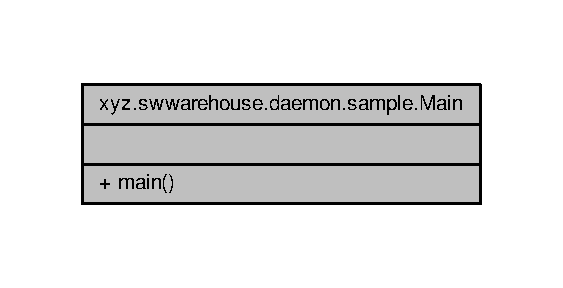
\includegraphics[width=286pt]{classxyz_1_1swwarehouse_1_1daemon_1_1sample_1_1_main__coll__graph}
\end{center}
\end{figure}
\subsection*{정적 Public 멤버 함수}
\begin{DoxyCompactItemize}
\item 
static void \hyperlink{classxyz_1_1swwarehouse_1_1daemon_1_1sample_1_1_main_a84f08835b7ba93a7adb60fa7479516a3}{main} (String\mbox{[}$\,$\mbox{]} args)
\begin{DoxyCompactList}\small\item\em run worker \end{DoxyCompactList}\end{DoxyCompactItemize}


\subsection{상세한 설명}
include main method 

\begin{DoxyAuthor}{작성자}
W\+E\+S 
\end{DoxyAuthor}
\begin{DoxyDate}{날짜}
2017-\/03-\/05 
\end{DoxyDate}
\begin{DoxyVersion}{버전}
1.\+0.\+0 
\end{DoxyVersion}


Main.\+java 파일의 14 번째 라인에서 정의되었습니다.



\subsection{멤버 함수 문서화}
\hypertarget{classxyz_1_1swwarehouse_1_1daemon_1_1sample_1_1_main_a84f08835b7ba93a7adb60fa7479516a3}{\index{xyz\+::swwarehouse\+::daemon\+::sample\+::\+Main@{xyz\+::swwarehouse\+::daemon\+::sample\+::\+Main}!main@{main}}
\index{main@{main}!xyz\+::swwarehouse\+::daemon\+::sample\+::\+Main@{xyz\+::swwarehouse\+::daemon\+::sample\+::\+Main}}
\subsubsection[{main}]{\setlength{\rightskip}{0pt plus 5cm}static void xyz.\+swwarehouse.\+daemon.\+sample.\+Main.\+main (
\begin{DoxyParamCaption}
\item[{String\mbox{[}$\,$\mbox{]}}]{args}
\end{DoxyParamCaption}
)\hspace{0.3cm}{\ttfamily [static]}}}\label{classxyz_1_1swwarehouse_1_1daemon_1_1sample_1_1_main_a84f08835b7ba93a7adb60fa7479516a3}


run worker 


\begin{DoxyParams}{매개변수}
{\em args} & \\
\hline
\end{DoxyParams}


Main.\+java 파일의 19 번째 라인에서 정의되었습니다.


\begin{DoxyCode}
19                                            \{
20         Worker worker = \textcolor{keyword}{new} Worker();
21         worker.run();
22     \}
\end{DoxyCode}


이 함수 내부에서 호출하는 함수들에 대한 그래프입니다.\+:\nopagebreak
\begin{figure}[H]
\begin{center}
\leavevmode
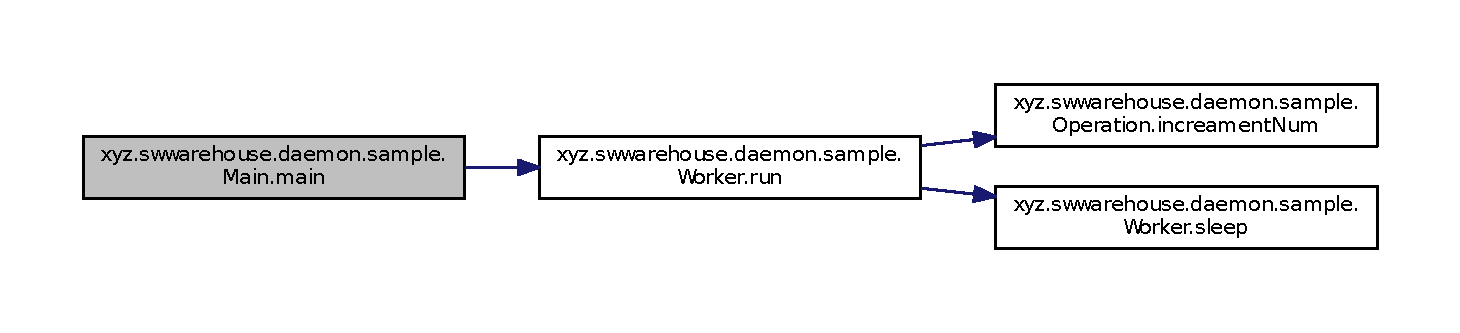
\includegraphics[width=350pt]{classxyz_1_1swwarehouse_1_1daemon_1_1sample_1_1_main_a84f08835b7ba93a7adb60fa7479516a3_cgraph}
\end{center}
\end{figure}




이 클래스에 대한 문서화 페이지는 다음의 파일로부터 생성되었습니다.\+:\begin{DoxyCompactItemize}
\item 
src/main/java/xyz/swwarehouse/daemon/sample/\hyperlink{_main_8java}{Main.\+java}\end{DoxyCompactItemize}

\hypertarget{classxyz_1_1swwarehouse_1_1daemon_1_1sample_1_1_operation}{\section{xyz.\-swwarehouse.\-daemon.\-sample.\-Operation 클래스 참조}
\label{classxyz_1_1swwarehouse_1_1daemon_1_1sample_1_1_operation}\index{xyz.\-swwarehouse.\-daemon.\-sample.\-Operation@{xyz.\-swwarehouse.\-daemon.\-sample.\-Operation}}
}


연산에 관한 함수를 포함하는 클래스  


\subsection*{Public 멤버 함수}
\begin{DoxyCompactItemize}
\item 
int \hyperlink{classxyz_1_1swwarehouse_1_1daemon_1_1sample_1_1_operation_a61a8a3f554babccb3b68a4ad16384d50}{increament\-Num} (int n)
\begin{DoxyCompactList}\small\item\em 정수(n)을 1씩 증가시키는 함수 \end{DoxyCompactList}\end{DoxyCompactItemize}


\subsection{상세한 설명}
연산에 관한 함수를 포함하는 클래스 

\begin{DoxyAuthor}{작성자}
W\-E\-S 
\end{DoxyAuthor}
\begin{DoxyVersion}{버전}
1.\-0.\-0 
\end{DoxyVersion}
\begin{DoxyDate}{날짜}
2017-\/03-\/05 
\end{DoxyDate}


Operation.\-java 파일의 8 번째 라인에서 정의되었습니다.



\subsection{멤버 함수 문서화}
\hypertarget{classxyz_1_1swwarehouse_1_1daemon_1_1sample_1_1_operation_a61a8a3f554babccb3b68a4ad16384d50}{\index{xyz\-::swwarehouse\-::daemon\-::sample\-::\-Operation@{xyz\-::swwarehouse\-::daemon\-::sample\-::\-Operation}!increament\-Num@{increament\-Num}}
\index{increament\-Num@{increament\-Num}!xyz::swwarehouse::daemon::sample::Operation@{xyz\-::swwarehouse\-::daemon\-::sample\-::\-Operation}}
\subsubsection[{increament\-Num}]{\setlength{\rightskip}{0pt plus 5cm}int xyz.\-swwarehouse.\-daemon.\-sample.\-Operation.\-increament\-Num (
\begin{DoxyParamCaption}
\item[{int}]{n}
\end{DoxyParamCaption}
)}}\label{classxyz_1_1swwarehouse_1_1daemon_1_1sample_1_1_operation_a61a8a3f554babccb3b68a4ad16384d50}


정수(n)을 1씩 증가시키는 함수 


\begin{DoxyParams}{매개변수}
{\em n} & \\
\hline
\end{DoxyParams}
\begin{DoxyReturn}{반환값}
n+1 
\end{DoxyReturn}


Operation.\-java 파일의 14 번째 라인에서 정의되었습니다.


\begin{DoxyCode}
14                                     \{
15         \textcolor{keywordflow}{return} n + 1;
16     \}
\end{DoxyCode}


이 함수를 호출하는 함수들에 대한 그래프입니다.\-:
\nopagebreak
\begin{figure}[H]
\begin{center}
\leavevmode
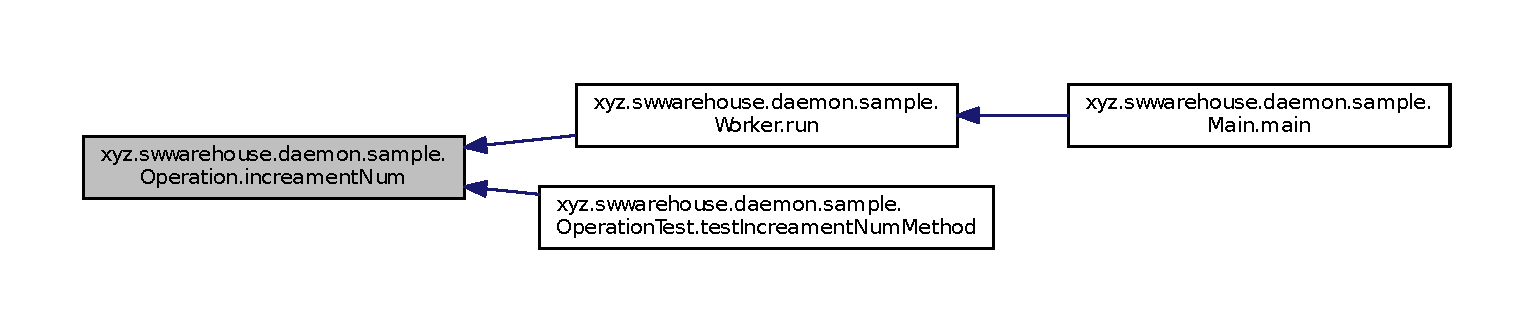
\includegraphics[width=350pt]{classxyz_1_1swwarehouse_1_1daemon_1_1sample_1_1_operation_a61a8a3f554babccb3b68a4ad16384d50_icgraph}
\end{center}
\end{figure}




이 클래스에 대한 문서화 페이지는 다음의 파일로부터 생성되었습니다.\-:\begin{DoxyCompactItemize}
\item 
src/main/java/xyz/swwarehouse/daemon/sample/\hyperlink{_operation_8java}{Operation.\-java}\end{DoxyCompactItemize}

\hypertarget{classxyz_1_1swwarehouse_1_1daemon_1_1sample_1_1_operation_test}{\section{xyz.\-swwarehouse.\-daemon.\-sample.\-Operation\-Test 클래스 참조}
\label{classxyz_1_1swwarehouse_1_1daemon_1_1sample_1_1_operation_test}\index{xyz.\-swwarehouse.\-daemon.\-sample.\-Operation\-Test@{xyz.\-swwarehouse.\-daemon.\-sample.\-Operation\-Test}}
}


\hyperlink{classxyz_1_1swwarehouse_1_1daemon_1_1sample_1_1_operation}{Operation} 클래스에 대한 단위테스트  


\subsection*{Public 멤버 함수}
\begin{DoxyCompactItemize}
\item 
void \hyperlink{classxyz_1_1swwarehouse_1_1daemon_1_1sample_1_1_operation_test_a64e62d430d25bd9177afb82935f0118a}{test\-Increament\-Num\-Method} ()
\begin{DoxyCompactList}\small\item\em Increament\-Num 함수에 대한 유닛테스트 \end{DoxyCompactList}\end{DoxyCompactItemize}


\subsection{상세한 설명}
\hyperlink{classxyz_1_1swwarehouse_1_1daemon_1_1sample_1_1_operation}{Operation} 클래스에 대한 단위테스트 

\begin{DoxyAuthor}{작성자}
W\-E\-S 
\end{DoxyAuthor}
\begin{DoxyVersion}{버전}
1.\-0.\-0 
\end{DoxyVersion}
\begin{DoxyDate}{날짜}
2017-\/03-\/05 
\end{DoxyDate}


Operation\-Test.\-java 파일의 16 번째 라인에서 정의되었습니다.



\subsection{멤버 함수 문서화}
\hypertarget{classxyz_1_1swwarehouse_1_1daemon_1_1sample_1_1_operation_test_a64e62d430d25bd9177afb82935f0118a}{\index{xyz\-::swwarehouse\-::daemon\-::sample\-::\-Operation\-Test@{xyz\-::swwarehouse\-::daemon\-::sample\-::\-Operation\-Test}!test\-Increament\-Num\-Method@{test\-Increament\-Num\-Method}}
\index{test\-Increament\-Num\-Method@{test\-Increament\-Num\-Method}!xyz::swwarehouse::daemon::sample::OperationTest@{xyz\-::swwarehouse\-::daemon\-::sample\-::\-Operation\-Test}}
\subsubsection[{test\-Increament\-Num\-Method}]{\setlength{\rightskip}{0pt plus 5cm}void xyz.\-swwarehouse.\-daemon.\-sample.\-Operation\-Test.\-test\-Increament\-Num\-Method (
\begin{DoxyParamCaption}
{}
\end{DoxyParamCaption}
)}}\label{classxyz_1_1swwarehouse_1_1daemon_1_1sample_1_1_operation_test_a64e62d430d25bd9177afb82935f0118a}


Increament\-Num 함수에 대한 유닛테스트 



Operation\-Test.\-java 파일의 21 번째 라인에서 정의되었습니다.


\begin{DoxyCode}
21                                           \{
22         Operation op = \textcolor{keyword}{new} Operation();
23         \textcolor{keywordtype}{int} n = 0;
24         assertEquals(n + 1, op.increamentNum(n));
25     \}
\end{DoxyCode}


이 함수 내부에서 호출하는 함수들에 대한 그래프입니다.\-:
\nopagebreak
\begin{figure}[H]
\begin{center}
\leavevmode
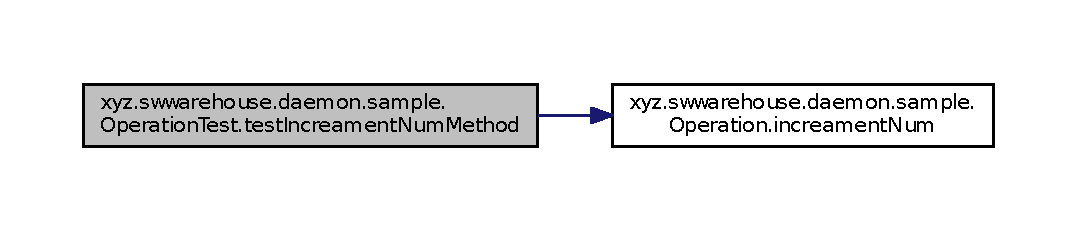
\includegraphics[width=350pt]{classxyz_1_1swwarehouse_1_1daemon_1_1sample_1_1_operation_test_a64e62d430d25bd9177afb82935f0118a_cgraph}
\end{center}
\end{figure}




이 클래스에 대한 문서화 페이지는 다음의 파일로부터 생성되었습니다.\-:\begin{DoxyCompactItemize}
\item 
src/test/java/xyz/swwarehouse/daemon/sample/\hyperlink{_operation_test_8java}{Operation\-Test.\-java}\end{DoxyCompactItemize}

\hypertarget{classxyz_1_1swwarehouse_1_1daemon_1_1sample_1_1_worker}{\section{xyz.\-swwarehouse.\-daemon.\-sample.\-Worker 클래스 참조}
\label{classxyz_1_1swwarehouse_1_1daemon_1_1sample_1_1_worker}\index{xyz.\-swwarehouse.\-daemon.\-sample.\-Worker@{xyz.\-swwarehouse.\-daemon.\-sample.\-Worker}}
}


데몬 클래스  




xyz.\-swwarehouse.\-daemon.\-sample.\-Worker에 대한 협력 다이어그램\-:
\nopagebreak
\begin{figure}[H]
\begin{center}
\leavevmode
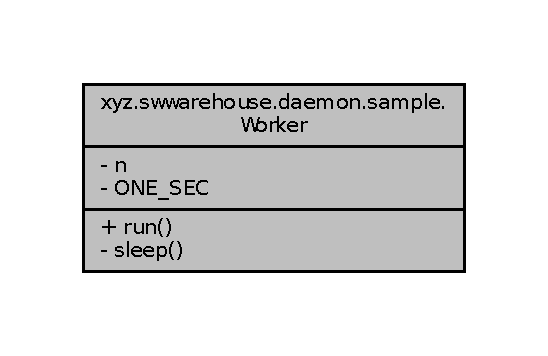
\includegraphics[width=250pt]{classxyz_1_1swwarehouse_1_1daemon_1_1sample_1_1_worker__coll__graph}
\end{center}
\end{figure}
\subsection*{Public 멤버 함수}
\begin{DoxyCompactItemize}
\item 
void \hyperlink{classxyz_1_1swwarehouse_1_1daemon_1_1sample_1_1_worker_af1bf199e3277a2946e59c7acc5416731}{run} ()
\begin{DoxyCompactList}\small\item\em 1초마다 n를 1씩 증가 시킨 후, 표준 출력. \end{DoxyCompactList}\end{DoxyCompactItemize}
\subsection*{Private 멤버 함수}
\begin{DoxyCompactItemize}
\item 
void \hyperlink{classxyz_1_1swwarehouse_1_1daemon_1_1sample_1_1_worker_ae9991783aa9ada529a18ecb5abdb4ad7}{sleep} (long term)
\begin{DoxyCompactList}\small\item\em try-\/catch 문을 포함한 sleep 함수 \end{DoxyCompactList}\end{DoxyCompactItemize}
\subsection*{Private 속성}
\begin{DoxyCompactItemize}
\item 
int \hyperlink{classxyz_1_1swwarehouse_1_1daemon_1_1sample_1_1_worker_aba3c26c1febb4e19bfc9562306bcee80}{n} = 0
\end{DoxyCompactItemize}
\subsection*{정적 Private 속성}
\begin{DoxyCompactItemize}
\item 
static final int \hyperlink{classxyz_1_1swwarehouse_1_1daemon_1_1sample_1_1_worker_a285c9ea5eebf4bb083140ca18048961a}{O\-N\-E\-\_\-\-S\-E\-C} = 1000
\end{DoxyCompactItemize}


\subsection{상세한 설명}
데몬 클래스 

\begin{DoxyAuthor}{작성자}
W\-E\-S 
\end{DoxyAuthor}
\begin{DoxyVersion}{버전}
1.\-0.\-0 
\end{DoxyVersion}
\begin{DoxyDate}{날짜}
2017-\/03-\/05 
\end{DoxyDate}


Worker.\-java 파일의 9 번째 라인에서 정의되었습니다.



\subsection{멤버 함수 문서화}
\hypertarget{classxyz_1_1swwarehouse_1_1daemon_1_1sample_1_1_worker_af1bf199e3277a2946e59c7acc5416731}{\index{xyz\-::swwarehouse\-::daemon\-::sample\-::\-Worker@{xyz\-::swwarehouse\-::daemon\-::sample\-::\-Worker}!run@{run}}
\index{run@{run}!xyz::swwarehouse::daemon::sample::Worker@{xyz\-::swwarehouse\-::daemon\-::sample\-::\-Worker}}
\subsubsection[{run}]{\setlength{\rightskip}{0pt plus 5cm}void xyz.\-swwarehouse.\-daemon.\-sample.\-Worker.\-run (
\begin{DoxyParamCaption}
{}
\end{DoxyParamCaption}
)}}\label{classxyz_1_1swwarehouse_1_1daemon_1_1sample_1_1_worker_af1bf199e3277a2946e59c7acc5416731}


1초마다 n를 1씩 증가 시킨 후, 표준 출력. 



Worker.\-java 파일의 16 번째 라인에서 정의되었습니다.


\begin{DoxyCode}
16                       \{
17         Operation op = \textcolor{keyword}{new} Operation();
18         \textcolor{keywordflow}{while} (\textcolor{keyword}{true}) \{
19             \hyperlink{classxyz_1_1swwarehouse_1_1daemon_1_1sample_1_1_worker_aba3c26c1febb4e19bfc9562306bcee80}{n} = op.increamentNum(\hyperlink{classxyz_1_1swwarehouse_1_1daemon_1_1sample_1_1_worker_aba3c26c1febb4e19bfc9562306bcee80}{n});
20             System.out.println(\hyperlink{classxyz_1_1swwarehouse_1_1daemon_1_1sample_1_1_worker_aba3c26c1febb4e19bfc9562306bcee80}{n});
21             \hyperlink{classxyz_1_1swwarehouse_1_1daemon_1_1sample_1_1_worker_ae9991783aa9ada529a18ecb5abdb4ad7}{sleep}(\hyperlink{classxyz_1_1swwarehouse_1_1daemon_1_1sample_1_1_worker_a285c9ea5eebf4bb083140ca18048961a}{ONE\_SEC});
22         \}
23     \}
\end{DoxyCode}


이 함수 내부에서 호출하는 함수들에 대한 그래프입니다.\-:
\nopagebreak
\begin{figure}[H]
\begin{center}
\leavevmode
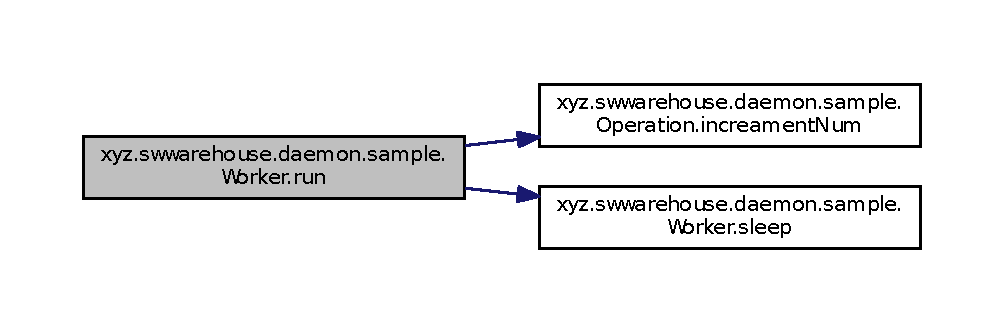
\includegraphics[width=350pt]{classxyz_1_1swwarehouse_1_1daemon_1_1sample_1_1_worker_af1bf199e3277a2946e59c7acc5416731_cgraph}
\end{center}
\end{figure}


\hypertarget{classxyz_1_1swwarehouse_1_1daemon_1_1sample_1_1_worker_ae9991783aa9ada529a18ecb5abdb4ad7}{\index{xyz\-::swwarehouse\-::daemon\-::sample\-::\-Worker@{xyz\-::swwarehouse\-::daemon\-::sample\-::\-Worker}!sleep@{sleep}}
\index{sleep@{sleep}!xyz::swwarehouse::daemon::sample::Worker@{xyz\-::swwarehouse\-::daemon\-::sample\-::\-Worker}}
\subsubsection[{sleep}]{\setlength{\rightskip}{0pt plus 5cm}void xyz.\-swwarehouse.\-daemon.\-sample.\-Worker.\-sleep (
\begin{DoxyParamCaption}
\item[{long}]{term}
\end{DoxyParamCaption}
)\hspace{0.3cm}{\ttfamily [private]}}}\label{classxyz_1_1swwarehouse_1_1daemon_1_1sample_1_1_worker_ae9991783aa9ada529a18ecb5abdb4ad7}


try-\/catch 문을 포함한 sleep 함수 


\begin{DoxyParams}{매개변수}
{\em term} & \\
\hline
\end{DoxyParams}


Worker.\-java 파일의 28 번째 라인에서 정의되었습니다.


\begin{DoxyCode}
28                                   \{
29         \textcolor{keywordflow}{try} \{
30             Thread.sleep(term);
31         \} \textcolor{keywordflow}{catch} (InterruptedException e) \{
32             \textcolor{comment}{// TODO Auto-generated catch block}
33             e.printStackTrace();
34         \}
35     \}
\end{DoxyCode}


이 함수를 호출하는 함수들에 대한 그래프입니다.\-:
\nopagebreak
\begin{figure}[H]
\begin{center}
\leavevmode
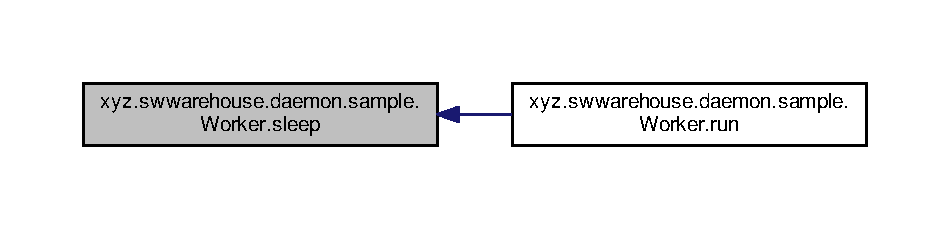
\includegraphics[width=350pt]{classxyz_1_1swwarehouse_1_1daemon_1_1sample_1_1_worker_ae9991783aa9ada529a18ecb5abdb4ad7_icgraph}
\end{center}
\end{figure}




\subsection{멤버 데이타 문서화}
\hypertarget{classxyz_1_1swwarehouse_1_1daemon_1_1sample_1_1_worker_aba3c26c1febb4e19bfc9562306bcee80}{\index{xyz\-::swwarehouse\-::daemon\-::sample\-::\-Worker@{xyz\-::swwarehouse\-::daemon\-::sample\-::\-Worker}!n@{n}}
\index{n@{n}!xyz::swwarehouse::daemon::sample::Worker@{xyz\-::swwarehouse\-::daemon\-::sample\-::\-Worker}}
\subsubsection[{n}]{\setlength{\rightskip}{0pt plus 5cm}int xyz.\-swwarehouse.\-daemon.\-sample.\-Worker.\-n = 0\hspace{0.3cm}{\ttfamily [private]}}}\label{classxyz_1_1swwarehouse_1_1daemon_1_1sample_1_1_worker_aba3c26c1febb4e19bfc9562306bcee80}


Worker.\-java 파일의 11 번째 라인에서 정의되었습니다.

\hypertarget{classxyz_1_1swwarehouse_1_1daemon_1_1sample_1_1_worker_a285c9ea5eebf4bb083140ca18048961a}{\index{xyz\-::swwarehouse\-::daemon\-::sample\-::\-Worker@{xyz\-::swwarehouse\-::daemon\-::sample\-::\-Worker}!O\-N\-E\-\_\-\-S\-E\-C@{O\-N\-E\-\_\-\-S\-E\-C}}
\index{O\-N\-E\-\_\-\-S\-E\-C@{O\-N\-E\-\_\-\-S\-E\-C}!xyz::swwarehouse::daemon::sample::Worker@{xyz\-::swwarehouse\-::daemon\-::sample\-::\-Worker}}
\subsubsection[{O\-N\-E\-\_\-\-S\-E\-C}]{\setlength{\rightskip}{0pt plus 5cm}final int xyz.\-swwarehouse.\-daemon.\-sample.\-Worker.\-O\-N\-E\-\_\-\-S\-E\-C = 1000\hspace{0.3cm}{\ttfamily [static]}, {\ttfamily [private]}}}\label{classxyz_1_1swwarehouse_1_1daemon_1_1sample_1_1_worker_a285c9ea5eebf4bb083140ca18048961a}


Worker.\-java 파일의 10 번째 라인에서 정의되었습니다.



이 클래스에 대한 문서화 페이지는 다음의 파일로부터 생성되었습니다.\-:\begin{DoxyCompactItemize}
\item 
src/main/java/xyz/swwarehouse/daemon/sample/\hyperlink{_worker_8java}{Worker.\-java}\end{DoxyCompactItemize}

\chapter{파일 문서화}
\hypertarget{_main_8java}{\section{src/main/java/xyz/swwarehouse/daemon/sample/\-Main.java 파일 참조}
\label{_main_8java}\index{src/main/java/xyz/swwarehouse/daemon/sample/\-Main.\-java@{src/main/java/xyz/swwarehouse/daemon/sample/\-Main.\-java}}
}
\subsection*{클래스}
\begin{DoxyCompactItemize}
\item 
class \hyperlink{classxyz_1_1swwarehouse_1_1daemon_1_1sample_1_1_main}{xyz.\-swwarehouse.\-daemon.\-sample.\-Main}
\begin{DoxyCompactList}\small\item\em include main method \end{DoxyCompactList}\end{DoxyCompactItemize}
\subsection*{패키지}
\begin{DoxyCompactItemize}
\item 
package \hyperlink{namespacexyz_1_1swwarehouse_1_1daemon_1_1sample}{xyz.\-swwarehouse.\-daemon.\-sample}
\end{DoxyCompactItemize}

\hypertarget{_operation_8java}{\section{src/main/java/xyz/swwarehouse/daemon/sample/\+Operation.java 파일 참조}
\label{_operation_8java}\index{src/main/java/xyz/swwarehouse/daemon/sample/\+Operation.\+java@{src/main/java/xyz/swwarehouse/daemon/sample/\+Operation.\+java}}
}
\subsection*{클래스}
\begin{DoxyCompactItemize}
\item 
class \hyperlink{classxyz_1_1swwarehouse_1_1daemon_1_1sample_1_1_operation}{xyz.\+swwarehouse.\+daemon.\+sample.\+Operation}
\begin{DoxyCompactList}\small\item\em 연산에 관한 함수를 포함하는 클래스 \end{DoxyCompactList}\end{DoxyCompactItemize}
\subsection*{패키지}
\begin{DoxyCompactItemize}
\item 
package \hyperlink{namespacexyz_1_1swwarehouse_1_1daemon_1_1sample}{xyz.\+swwarehouse.\+daemon.\+sample}
\end{DoxyCompactItemize}

\hypertarget{_worker_8java}{\section{src/main/java/xyz/swwarehouse/daemon/sample/\+Worker.java 파일 참조}
\label{_worker_8java}\index{src/main/java/xyz/swwarehouse/daemon/sample/\+Worker.\+java@{src/main/java/xyz/swwarehouse/daemon/sample/\+Worker.\+java}}
}
\subsection*{클래스}
\begin{DoxyCompactItemize}
\item 
class \hyperlink{classxyz_1_1swwarehouse_1_1daemon_1_1sample_1_1_worker}{xyz.\+swwarehouse.\+daemon.\+sample.\+Worker}
\begin{DoxyCompactList}\small\item\em 데몬 클래스 \end{DoxyCompactList}\end{DoxyCompactItemize}
\subsection*{패키지}
\begin{DoxyCompactItemize}
\item 
package \hyperlink{namespacexyz_1_1swwarehouse_1_1daemon_1_1sample}{xyz.\+swwarehouse.\+daemon.\+sample}
\end{DoxyCompactItemize}

\hypertarget{_operation_test_8java}{\section{src/test/java/xyz/swwarehouse/daemon/sample/\-Operation\-Test.java 파일 참조}
\label{_operation_test_8java}\index{src/test/java/xyz/swwarehouse/daemon/sample/\-Operation\-Test.\-java@{src/test/java/xyz/swwarehouse/daemon/sample/\-Operation\-Test.\-java}}
}
\subsection*{클래스}
\begin{DoxyCompactItemize}
\item 
class \hyperlink{classxyz_1_1swwarehouse_1_1daemon_1_1sample_1_1_operation_test}{xyz.\-swwarehouse.\-daemon.\-sample.\-Operation\-Test}
\begin{DoxyCompactList}\small\item\em \hyperlink{classxyz_1_1swwarehouse_1_1daemon_1_1sample_1_1_operation}{Operation} 클래스에 대한 단위테스트 \end{DoxyCompactList}\end{DoxyCompactItemize}
\subsection*{패키지}
\begin{DoxyCompactItemize}
\item 
package \hyperlink{namespacexyz_1_1swwarehouse_1_1daemon_1_1sample}{xyz.\-swwarehouse.\-daemon.\-sample}
\end{DoxyCompactItemize}

%--- End generated contents ---

% Index
\newpage
\phantomsection
\addcontentsline{toc}{part}{색인}
\printindex

\end{document}
